\section{Muon system}

\subsection{Muon Spectrometer}

%\subsubsection{Motivation}
The tracking system determines the transverse momentum of a charged particle from its radius of curvature in a magnetic field since $R = p_T /(qB)$.  A more massive object moving at the same velocity will have a larger transverse momentum, and therefore a larger radius of curvature.  Since the muon is 200 times heavier than an electron, it can be difficult to have a tracking system that can accurately measure the momentum for relativistic muons and electrons, so the muon detection system is distinct to measure the $p_T$ for a broad range of muon energies.  

The muon detector is a gas detector like the TRT, and operates according to similar principles. 
The subsections below detail the components of the muon spectrometer, while the parameters for the coverage and number of channels for are listed in \Fig{Muon-table}.

\begin{figure}[h!tbp]
\centering
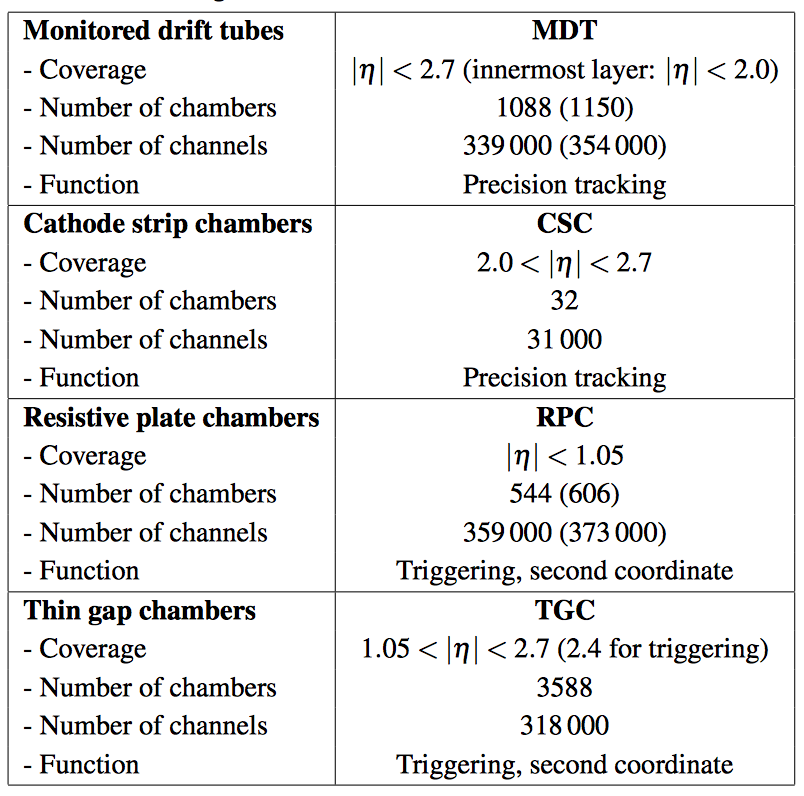
\includegraphics[width=0.75\textwidth]{\figpath/Muon_table.png}
\caption{Main parameters for the Muon Spectrometer.  The values in parentheses refer to the configuration from 2009~\cite{ATLAS_long}.}
\label{Muon-table}
\end{figure}

\subsubsection{Toroidal Magnets}

The muons are detected through the deflection of their tracks in a 4~T magnetic field.  There are three large air--core toroids, and each of these 3 toroids has 8 coils.  
The particles of interest that reach this portion of the detector are muons and neutrinos, but only the muons will be detected because the electrically neutral neutrinos are not deflected by the magnetic field.  
Backgrounds for the muon spectrometer are photons and neutrons with energies below an MeV and 100~MeV, respectively \cite{ATLAS_long}.  
The magnetic field is designed to be transverse to the muons' flight direction to minimize multiple scattering. The magnets are housed within cryostats to keep them below the critical temperature for superconductivity.  Inside these magnets are the muon chambers divided into three cylindrical chambers about the beam axis in the barrel region, while the transition and end--cap regions arranged as disks, also divided into three chambers \cite{ATLAS_long}.

\subsubsection{Monitored Drift Tubes}

The Monitored Drift Tubes (MDTs) are drift chambers that provide precision measurements. Each tube is made of aluminum with a 3~cm diameter and length between 0.9 and 6.2~m.  
The tube is filled with a 93\%~Ar,~7\%~CO$_2$ gas mixture, at a pressure of 3-bar \cite{ATLAS_long}.  It has a gain of $2\times10^4$ \cite{ATLAS_long}, similar to the TRT drift chambers (see \Section{trt}). The precision for single muon events is 100~$\mu$m, while the precision for multi-muon events is 50~$\mu$m \cite{ATLAS_long}. To control the precision, the sag of the wires is minimized by three kinematical mounts placed strategically to minimize distortion due to the support, as shown in \Fig{MDT-alignment}. There are a total of 1174 MDTs positioned in the barrel of the ATLAS detector ($|\eta| < 2$).

\begin{figure}[h!tbp]
	\centering
	\subfloat[Illustration of how an MDT works ~\cite{ATLAS_long}.]{
	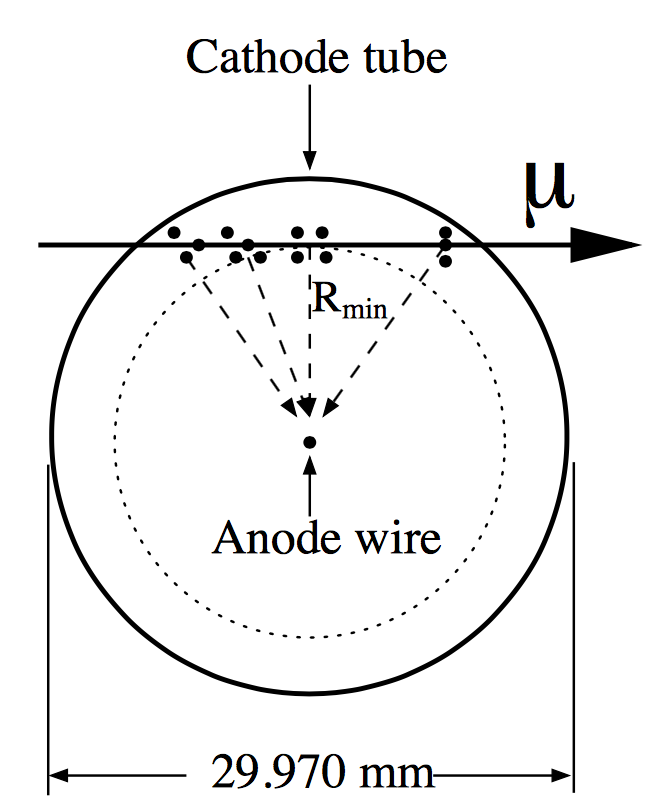
\includegraphics[width=0.25\textwidth]{\figpath/MDT_cartoon.png}
	\label{MDT_cartoon}
	}
	\subfloat[The orientation of the multi-layer MDT chamber with the support structure~\cite{ATLAS_long}.]{
	\includegraphics[[width=0.65\textwidth]{\figpath/MDT-alignment.png}
	\label{MDT_alignment}
	}
\caption{Monitored Drift Tubes: MDTs}
\end{figure}

\subsection{Cathode Strip Chambers}
\label{cdc}
For larger pseudorapidities ($2 < |\eta| < 2.7$), Cathode Strip Chambers (CSCs) are used for their higher granularity in the endcap region \cite{ATLAS_long}.  This is a multi-wire proportional chamber with strip read--out with a sense wire pitch of 2.54~mm and a read--out strip pitch of 5.08~mm resulting in a 60~$\mu$m track resolution \cite{ATLAS_long}.  
